%%

Weakly supervised object localization and learning
(WSL)~\cite{Wang:2014tg,Cinbis:2015wn} is the problem of localizing spatial
extents of target objects and learning their representations from a dataset with
only image-level labels. %%
%%
WSL is motivated by two fundamental issues of conventional object recognition.
First, the strong supervision in terms of object bounding boxes or segmentation
masks is difficult to obtain and prevents scaling-up object localization to
thousands of object classes. Second, imprecise and ambiguous manual annotations
can introduce subjective biases to the learning. 
%%
%%
%%
Convolutional neural networks (CNN)~\cite{LeCun:1989bx,Krizhevsky:2012wl}
have recently taken over the state of the art in many computer vision tasks.
CNN-based methods for weakly supervised object localization have been explored
in~\cite{Oquab:2015us,Bilen:2015uo}.
%%
Despite this progress, WSL remains a very challenging problem. The state-of-the-art performance
of WSL on standard benchmarks~\cite{Wang:2014tg,Cinbis:2015wn,Bilen:2015uo} is considerably lower compared to the
strongly supervised counterparts~\cite{Girshick:2016ig,ren15fasterrcnn,Gidaris:2015cx}. 

%%
%%

Strongly supervised detection methods often use contextual information from regions around the object or from the whole 
image~\cite{Torralba:2003wk,Rabinovich:2007wy,Felzenszwalb:2009wx,Girshick:2016ig,Gidaris:2015cx, desai09}:
Indeed, visual context often provides useful information about which image regions are likely to
be a target class according to object-background or object-object relations,
e.g., a boat in the sea, a bird in the sky, a person on a horse, a table around
a chair, etc. However, can a similar effect be achieved for object localization
in a weakly supervised setting, where training data does not contain any
supervisory information neither about object locations nor about context regions?

\begin{figure}[t] 
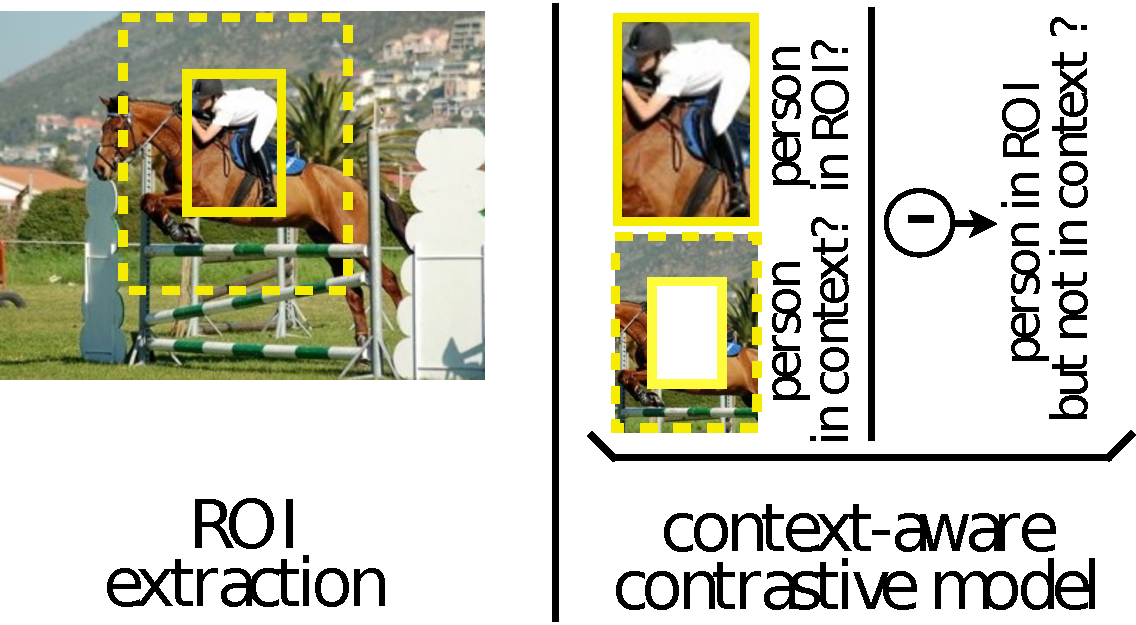
\includegraphics[width=\textwidth, trim={2mm 6.0cm 2mm 3cm},
clip]{images/overview} 
\vspace{-6ex} 
\caption[small]{Context-aware guidance for weakly supervised detection.
Given extracted ROIs as localization candidates, our two basic context-aware models, {\em additive} and {\em contrastive} models, leverage their surrounding context regions to improve localization. The additive model relies on semantic consistency that aggregates  class activations from ROI and context. The contrastive model relies on semantic contrast that computes  difference of class activations between ROI and context. For details, see text. (Best viewed in color.)} 
\label{fig:intro} 
\end{figure}

%%
%%
%%
The main contribution of this paper is exploring the use of context as a
supervisory guidance for WSL with CNNs. In a nutshell, we show that, even without strong
supervision, visual context can guide localization in two ways: {\it additive
} and {\it contrastive} guidances.  As the conventional use of contextual
information, the additive guidance enforces the predicted object region to be
compatible with its surrounding context region. This can be encoded by
maximizing the sum of a class score of a candidate region with that of its
surrounding context.
On the other hand, the contrastive guidance encourages the
predicted object region to be outstanding from its surrounding context region.
This can be encoded by maximizing the difference between a class score of the
object region and that of the surrounding context. %%
%%
For example, let us consider a candidate box for a person and its surrounding
region of context in Fig.~\ref{fig:intro}. In additive guidance,
appearance of a horse in the surrounding context helps us infer the
surrounded region to contain a person. In contrast guidance, the absence of
target-specific (person) features in its surrounding context helps 
separating the object region from its background.

%%
%%
%%

In this work, we introduce two types of CNN architectures, {\it additive} and
{\it contrastive} models, corresponding to the two contextual guidances. 
Building on the efficient region-of-interest (ROI) pooling
architecture~\cite{ren15fasterrcnn}, the proposed models capture effective
features among potential context regions to localize objects and learn their
representations.
In practice we observe that our additive model prevents expansion of detections
beyond object boundaries. On the other hand, the contrastive model prevents
contraction of detections to small object parts.
In experimental evaluation, we show that our models
significantly outperform the baselines and demonstrate effectiveness of our models for WSL. The project webpage and the code is available at \url{http://www.di.ens.fr/willow/research/contextlocnet}.